\documentclass[11pt,fleqn]{article}

\setlength {\topmargin} {-.15in}
\setlength {\textheight} {8.6in}

\usepackage{amsmath}
\usepackage{amssymb}
\usepackage{color}
\usepackage{tikz}
\usetikzlibrary{automata,positioning,arrows}
\usepackage{diagbox}
\usepackage{stackrel}
\begin{document}


\textbf{1.4.17} Farthest pair (in one dimension). Write a program that, given an array a[] of N
double values, finds a farthest pair : two values whose difference is no smaller than the
the difference of any other pair (in absolute value). The running time of your program
should be $linear$ in the worst case.\\

\textbf{Solution:}
One soln could be to sort the array if unsorted, then subtract end index(largest num) with start index(smallest num). This requires $nlogn$ complexity to sort the array first with fastest available sorting algo. This is linearithmic, not linear. We need linear soln. \\

A soln with $O(N)$ complexity would be to run through the array to find min and max, which will represent the pair with farthest distance.\\

\begin{center}
	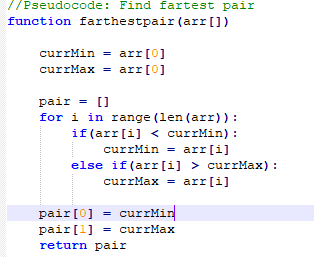
\includegraphics[scale = 1]{1.4.17.png}
	\end{center}

\end{document}
